%-*-latex-*-
\begin{center}
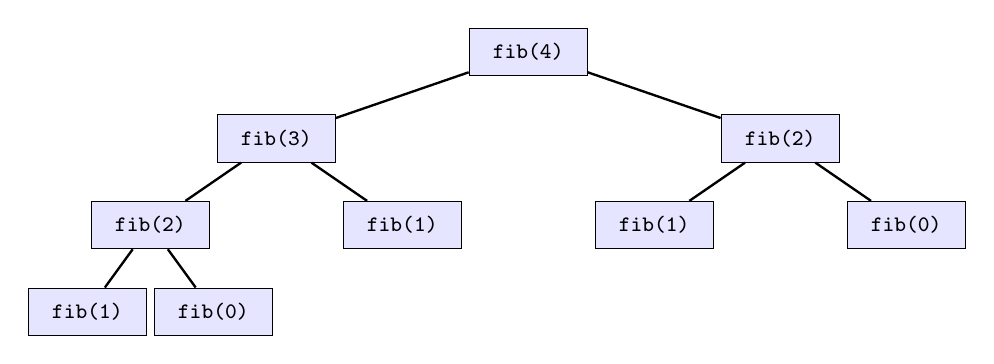
\begin{tikzpicture}

\draw (6.3500000000000005, 0.3)
  node[fill=blue!10,rounded corners=0cm,inner sep=0cm] {

\begin{minipage}[t][0.6cm]{1.5cm}
\mbox{}

\end{minipage}

};
\draw (6.3500000000000005, 0.3)
  node[draw, , , color=black,
       rounded corners=0cm, inner sep=0cm,
       name=A] {

\begin{minipage}[t][0.6cm]{1.5cm}
\mbox{}

\end{minipage}

};\draw (6.3500000000000005, 0.3) node[color=black] {\texttt{{\footnotesize \texttt{fib(4)}}}};
\draw (3.1500000000000004, -0.8)
  node[fill=blue!10,rounded corners=0cm,inner sep=0cm] {

\begin{minipage}[t][0.6cm]{1.5cm}
\mbox{}

\end{minipage}

};
\draw (3.1500000000000004, -0.8)
  node[draw, , , color=black,
       rounded corners=0cm, inner sep=0cm,
       name=B] {

\begin{minipage}[t][0.6cm]{1.5cm}
\mbox{}

\end{minipage}

};\draw (3.1500000000000004, -0.8) node[color=black] {\texttt{{\footnotesize \texttt{fib(3)}}}};
\draw (9.55, -0.8)
  node[fill=blue!10,rounded corners=0cm,inner sep=0cm] {

\begin{minipage}[t][0.6cm]{1.5cm}
\mbox{}

\end{minipage}

};
\draw (9.55, -0.8)
  node[draw, , , color=black,
       rounded corners=0cm, inner sep=0cm,
       name=I] {

\begin{minipage}[t][0.6cm]{1.5cm}
\mbox{}

\end{minipage}

};\draw (9.55, -0.8) node[color=black] {\texttt{{\footnotesize \texttt{fib(2)}}}};
\draw (1.5499999999999998, -1.9000000000000001)
  node[fill=blue!10,rounded corners=0cm,inner sep=0cm] {

\begin{minipage}[t][0.6cm]{1.5cm}
\mbox{}

\end{minipage}

};
\draw (1.5499999999999998, -1.9000000000000001)
  node[draw, , , color=black,
       rounded corners=0cm, inner sep=0cm,
       name=C] {

\begin{minipage}[t][0.6cm]{1.5cm}
\mbox{}

\end{minipage}

};\draw (1.5499999999999998, -1.9000000000000001) node[color=black] {\texttt{{\footnotesize \texttt{fib(2)}}}};
\draw (4.75, -1.9000000000000001)
  node[fill=blue!10,rounded corners=0cm,inner sep=0cm] {

\begin{minipage}[t][0.6cm]{1.5cm}
\mbox{}

\end{minipage}

};
\draw (4.75, -1.9000000000000001)
  node[draw, , , color=black,
       rounded corners=0cm, inner sep=0cm,
       name=F] {

\begin{minipage}[t][0.6cm]{1.5cm}
\mbox{}

\end{minipage}

};\draw (4.75, -1.9000000000000001) node[color=black] {\texttt{{\footnotesize \texttt{fib(1)}}}};
\draw (7.949999999999999, -1.9000000000000001)
  node[fill=blue!10,rounded corners=0cm,inner sep=0cm] {

\begin{minipage}[t][0.6cm]{1.5cm}
\mbox{}

\end{minipage}

};
\draw (7.949999999999999, -1.9000000000000001)
  node[draw, , , color=black,
       rounded corners=0cm, inner sep=0cm,
       name=G] {

\begin{minipage}[t][0.6cm]{1.5cm}
\mbox{}

\end{minipage}

};\draw (7.949999999999999, -1.9000000000000001) node[color=black] {\texttt{{\footnotesize \texttt{fib(1)}}}};
\draw (11.15, -1.9000000000000001)
  node[fill=blue!10,rounded corners=0cm,inner sep=0cm] {

\begin{minipage}[t][0.6cm]{1.5cm}
\mbox{}

\end{minipage}

};
\draw (11.15, -1.9000000000000001)
  node[draw, , , color=black,
       rounded corners=0cm, inner sep=0cm,
       name=H] {

\begin{minipage}[t][0.6cm]{1.5cm}
\mbox{}

\end{minipage}

};\draw (11.15, -1.9000000000000001) node[color=black] {\texttt{{\footnotesize \texttt{fib(0)}}}};
\draw (0.75, -3.0)
  node[fill=blue!10,rounded corners=0cm,inner sep=0cm] {

\begin{minipage}[t][0.6cm]{1.5cm}
\mbox{}

\end{minipage}

};
\draw (0.75, -3.0)
  node[draw, , , color=black,
       rounded corners=0cm, inner sep=0cm,
       name=D] {

\begin{minipage}[t][0.6cm]{1.5cm}
\mbox{}

\end{minipage}

};\draw (0.75, -3.0) node[color=black] {\texttt{{\footnotesize \texttt{fib(1)}}}};
\draw (2.35, -3.0)
  node[fill=blue!10,rounded corners=0cm,inner sep=0cm] {

\begin{minipage}[t][0.6cm]{1.5cm}
\mbox{}

\end{minipage}

};
\draw (2.35, -3.0)
  node[draw, , , color=black,
       rounded corners=0cm, inner sep=0cm,
       name=E] {

\begin{minipage}[t][0.6cm]{1.5cm}
\mbox{}

\end{minipage}

};\draw (2.35, -3.0) node[color=black] {\texttt{{\footnotesize \texttt{fib(0)}}}};\draw[line width=0.03cm,black] (A) to  (B);
\draw[line width=0.03cm,black] (A) to  (I);
\draw[line width=0.03cm,black] (B) to  (C);
\draw[line width=0.03cm,black] (B) to  (F);
\draw[line width=0.03cm,black] (C) to  (D);
\draw[line width=0.03cm,black] (C) to  (E);
\draw[line width=0.03cm,black] (I) to  (G);
\draw[line width=0.03cm,black] (I) to  (H);
\end{tikzpicture}

\end{center}

